\documentclass[10pt]{article}
\usepackage{amsmath,textcomp,amssymb,graphicx}
\usepackage[margin=0.45in]{geometry}
\title{Homework 1 Write-Up}
\date{01/31/2014}
\author{Alexander Chu}
\begin{document}
\maketitle
\section{Problem 1}
\begin{center}
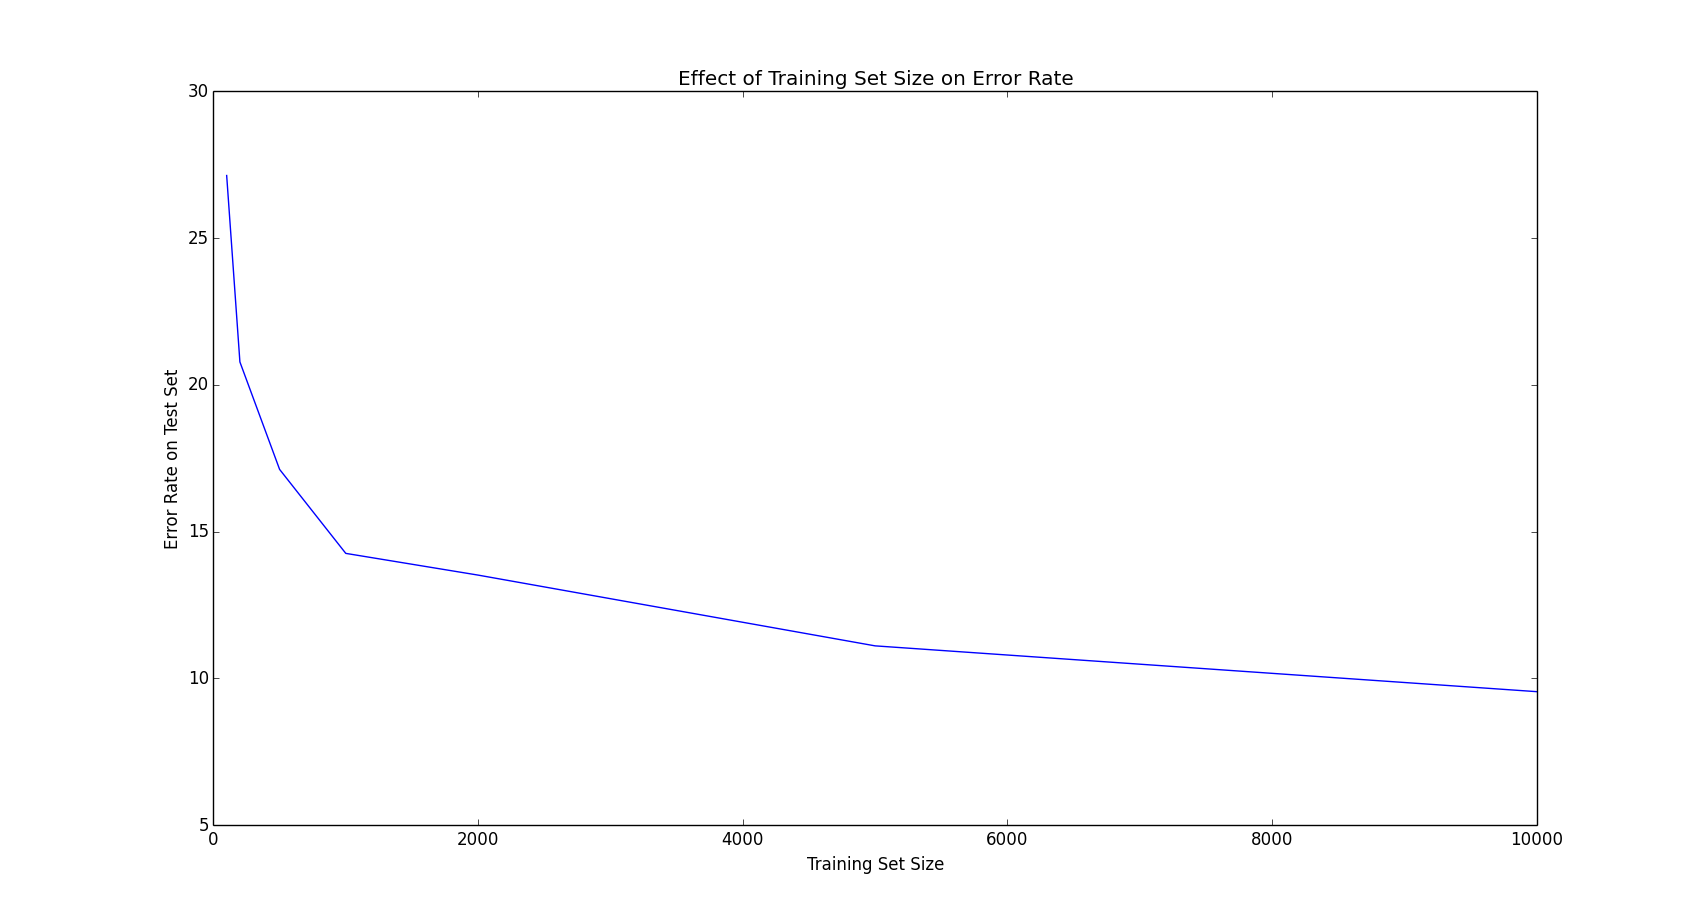
\includegraphics[scale=.5]{./errorPlot.png}
\end{center}
As shown in the plot, error decreases exponentially with increasing training set size.
To train the SVM, we used parameters \begin{verbatim}-B 10000 -c 0.001 -s 2\end{verbatim}, which denotes a Bias of 10000, a Cost of 0.001, and L2-regularized L2-loss support vector classification. These parameters were chosen based on our results from Problem 3, in which we tried values [1, 10, 100, 1000, 10000, 100000] for bias and values [0.1, 0.01, 0.001, 0.0001] for Cost.
\section{Problem 2}
\begin{center}
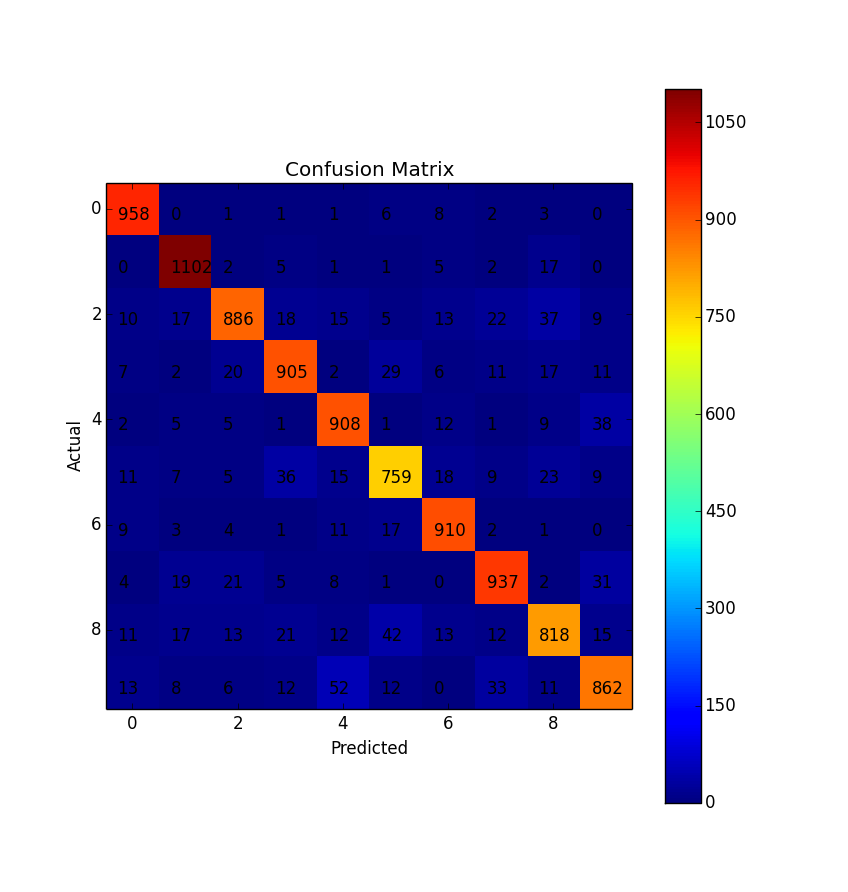
\includegraphics[scale=.8]{./confusionMatrix.png}
\end{center}
From the confusion matrix, we can deduce some of the more common errors produced by the SVM\. For instance, the most common mistake our SVM made in the test set was mistaking a 9 for a 4. Other common errors include mistaking a 8 for a 5, and a 5 for a 3. Errors were often reciprocal (the number of mistakes between 5 and 8 is similar to the number of mistakes between 8 and 5), and none of them were particularly asymmetric. The SVM's worst performance was on 5, which makes sense, since it bears pixel-wise similarities to numbers like 2,3, and 8. The confusion matrix provides insight as to how one might design a better feature space that caters specifically to these errors.
\section{Problem 3}
Cross validation helps give an accurate gauge of model accuracy. By holding out a segment of the training data and testing on it, cross validation simulates tests on real world data. This prevents over-fitting and provides a better litmus as to which set of hyper-parameter values produces the optimal results. K-fold cross validation is simply a more robust version of cross validation that symmetrically holds each partition of the dataset as the held-out set, providing an even better measure of the level of over-fitting. 
From our cross-validation, the optimal value of $c$ is 0.01, yielding a test error rate of 9.55\%.
\end{document}
